\documentclass[12pt]{article}
\usepackage{graphicx}
%\documentclass[journal,12pt,twocolumn]{IEEEtran}
\usepackage[none]{hyphenat}
\usepackage{graphicx}
\usepackage{listings}
\usepackage[english]{babel}
\usepackage{graphicx}
\usepackage{caption}
\usepackage[parfill]{parskip}
\usepackage{hyperref}
\usepackage{gensymb}
\usepackage{booktabs}
%\usepackage{setspace}\doublespacing\pagestyle{plain}
\def\inputGnumericTable{}
\usepackage{color}                                            %%
    \usepackage{array}                                            %%
    \usepackage{longtable}                                        %%
    \usepackage{calc}                                             %%
    \usepackage{multirow}                                         %%
    \usepackage{hhline}                                           %%
    \usepackage{ifthen}
\usepackage{array}
\usepackage{amsmath}   % for having text in math mode
\usepackage{parallel,enumitem}
\usepackage{listings}
\lstset{
language=tex,
frame=single,
breaklines=true
}
 
%Following 2 lines were added to remove the blank page at the beginning
\usepackage{atbegshi}% http://ctan.org/pkg/atbegshi
\AtBeginDocument{\AtBeginShipoutNext{\AtBeginShipoutDiscard}}
%
%New macro definitions
\newcommand{\mydet}[1]{\ensuremath{\begin{vmatrix}#1\end{vmatrix}}}
\providecommand{\brak}[1]{\ensuremath{\left(#1\right)}}
\providecommand{\norm}[1]{\left\lVert#1\right\rVert}
\newcommand{\solution}{\noindent \textbf{Solution: }}
\newcommand{\myvec}[1]{\ensuremath{\begin{pmatrix}#1\end{pmatrix}}}
\providecommand{\abs}[1]{\left\vert#1\right\vert}
\let\vec\mathbf
\begin{document}
\begin{center}
\enlargethispage{-4cm}
\title{\textbf{Circles}}
\date{\vspace{-5ex}} %Not to print date automatically
\maketitle
\end{center}
\setcounter{page}{1}
\section*{10$^{th}$ Maths - Chapter 10}
This is Problem-3 from Exercise 1
\begin{enumerate}
	\item A tangent $\vec{PQ}$ at a point $\vec{P}$ of a circle of radius 5 cm meets a line through the centre $\vec{O}$ at a point $\vec{Q}$ so that $\vec{OQ}$ = 12 cm. Length $\vec{PQ}$ is

\solution Given,
		\begin{align}
			\vec{OP}&=5cm\\
			\vec{OQ}&=12cm
		\end{align}
		As $\vec{OP}\perp\vec{PQ}$ then $\vec{OPQ}$ forms as a right triangle
		\begin{align}
\vec{OQ}^2&=\vec{OP}^2+\vec{PQ}^2\\
\vec{PQ}^2&=144-25\\
\vec{PQ}&=\sqrt{119}
		\end{align}
\begin{figure}[!h]
\begin{center}
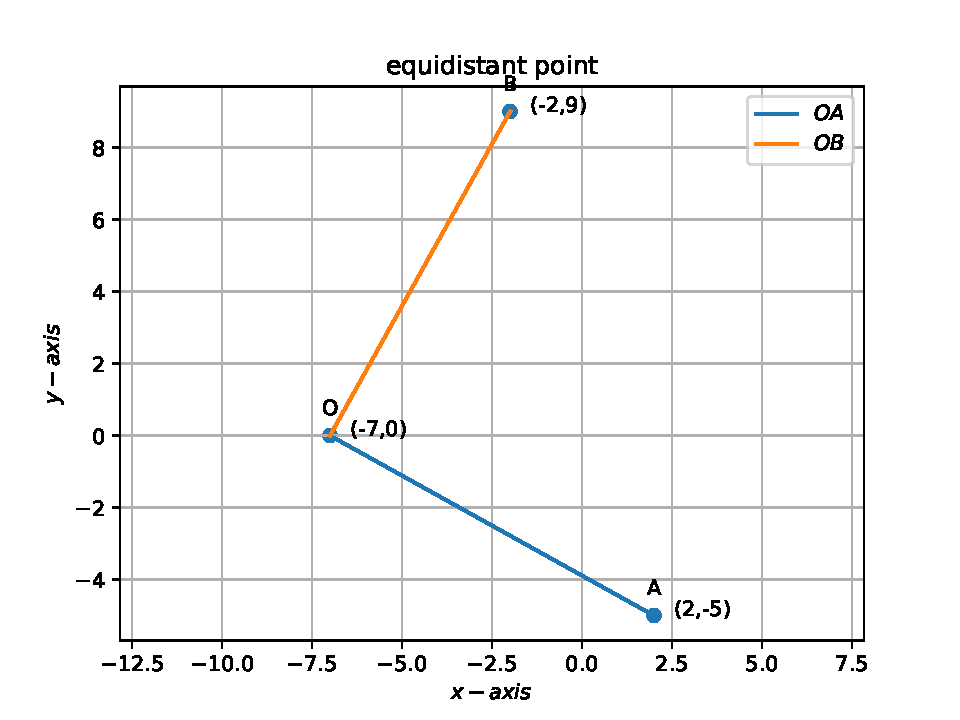
\includegraphics[width=\columnwidth]{figs/fig.pdf}
\end{center}
\caption{}
\label{fig:Fig1}
\end{figure}
\end{enumerate}
\end{document}
